\documentclass[10pt,a4paper]{article}
\usepackage[utf8]{inputenc}
\usepackage[ngerman]{babel}
\usepackage[T1]{fontenc}
\usepackage{amsmath}
\usepackage{amsfonts}
\usepackage{amssymb}
\usepackage{graphicx}
\usepackage{lmodern}
\usepackage{physics}
\usepackage[left=1cm,right=1cm,top=2cm,bottom=1.5cm]{geometry}
\usepackage{siunitx}
\usepackage{fancyhdr}
\usepackage{enumerate}
\usepackage{mhchem}
\usepackage{mathtools}
\usepackage{graphicx}
\graphicspath{./Figures}
\usepackage{float}
\usepackage{xcolor}
\usepackage{mdframed}
\usepackage{csquotes}
\usepackage{trfsigns}
\usepackage{capt-of}
\usepackage{listings}

\sisetup{locale=DE}
\sisetup{per-mode = symbol-or-fraction}
\sisetup{separate-uncertainty=true}
\DeclareSIUnit\year{a}
\DeclareSIUnit\clight{c}
\mdfdefinestyle{exercise}{
	backgroundcolor=black!10,roundcorner=8pt,hidealllines=true,nobreak
}

\begin{document}
\twocolumn
\pagestyle{fancy}
\lhead{Regelungstechnik \\ Formelsammlung}
\rhead{\today \\ Maximilian, Binninger}
\section{Grundlagen}
  \subsection{Eigenschaften}
  Eigenschaften LTI-Systeme
  \begin{mdframed}[style=exercise]
    \begin{enumerate}
      \item Stabilität\\
      $\abs{x(t)} < M < \infty \Rightarrow \abs{y(t)} < N < \infty$
      \item Linearität\\
          $W\qty{\sum_{k=1}^{N}a_n x_n(t)}=\sum_{n=1}^{N}W\qty{a_n x_n(t)}$
      \item Zeitinvarianz\\
      $W\qty{x(t-t_0)} =y(t-t_0)$
      \item Kausalität\\
      $t < 0 \Rightarrow x(t)=0 \land y(t)=0$
    \end{enumerate}
  \end{mdframed}
  \subsection{Systemantwort}
  Die Sprung-/Impulsantwort beschreibt Systemantwort vollständig
  \begin{mdframed}[style=exercise]
    \begin{align}
      y(t) &= \int^{\infty}_{-\infty} a(t-\tau) x'(\tau) \dd{\tau}\\
      a(t-\tau) &= W\qty{s(t-\tau)}\nonumber
    \end{align}
  \end{mdframed}
  \begin{mdframed}[style=exercise]
    \begin{align}
      y(t) &= \int_{-\infty}^{\infty} h(t-\tau) x(\tau) \dd{\tau}\\
      h(t-\tau) &= W\qty{\delta(t-\tau)}\nonumber
    \end{align}
  \end{mdframed}
  \subsection{Abtasttheorem}
  Durch die Abtastung wird das Spektrum von $f(t)$ unendlich oft um die Frequenzen $n\cdot \omega_a$ reproduziert.
  \begin{mdframed}[style=exercise]
    \begin{align}
      F_A(\omega) &= \frac{1}{T_A} \sum_{n=-\infty}^{\infty} F(\omega-n\omega_A)\\
      2\omega_g &\leq \omega_A\nonumber
    \end{align}
  \end{mdframed}
  \section{Systemtechnik}
  \subsection{Modellbildung}
  Hinweise zum aufstellen der Differentialgleichung eines Systems:
  \begin{mdframed}[style=exercise]
  \begin{enumerate}
      \item Bestimmmung der Ein- und Ausgangsgrößen
      \item Suche nach dem beschreibenden Gleichgewicht
      \item In der Gleichung dürfen nur Konstanten, sowie die Ein- und
          Augangsgrorßen in beliebiger Ableitung vorkommen
      \item Andere Variablen müssen durch erlaubte Größen ersetzt werden (Dazu
          können i.a. physikalische Gleichungen benutzt werden)
    \end{enumerate}
\end{mdframed}
\subsection{Signalflussplan/Blockschaltbild}
    Erzeugung des Signalflussplans aus der Zugehörigen DGL.
    \begin{mdframed}[style=exercise]
        \begin{enumerate}
                für technische Realissierung gilt: m < n;\\
                Dgl. nach höchster Ableitung der Ausgangsgröße auflösen\\
                höchste Ableitung der Ausgangsgröße geht auf den Eingan des ersten Integrators\\
                (Laplace-Trans ersetzt das Intergrieren mit einer Division mit „s“)\\
        \end{enumerate}
    \end{mdframed}
    \begin{center}
            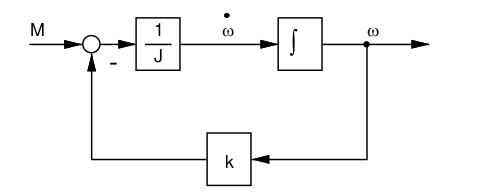
\includegraphics[width=.30\textwidth]{Figures/Signalflussplan12.png}
        \end{center}
        Erzeugung des Signalflussplans eines Systems mit der Dgl.:
        \begin{center}
                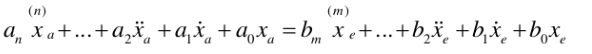
\includegraphics[width=.45\textwidth]{Figures/DGLSF.png}
        \end{center}
                Signalflussplan kann allgemein gezeichnet werden:\\
        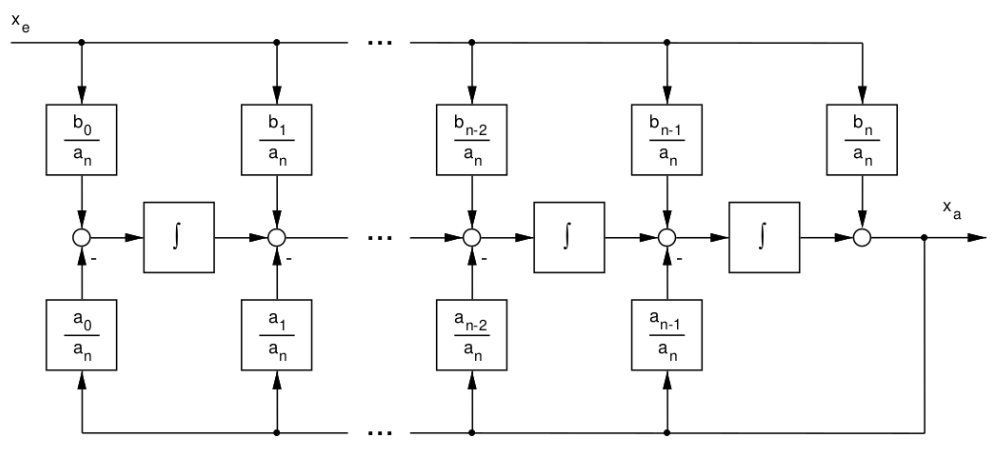
\includegraphics[width=.5\textwidth]{Figures/SFmitDGL.png}
\subsection{Stabilität}
    \begin{mdframed}[style=exercise]
    BIBO-Stabiliät (Bounded Input/ Bounded Output-> begrenzt):\\
    ein dynamisches System ist stabil, wenn gilt:\\
    für ein begrenztes $x_e$ gibt es immer ein begrenztes $x_a$
\end{mdframed}
\subsection{Ortskurven und Frequenzkennlinien}
    Ortskurvendarstellung:
    \begin{center}
    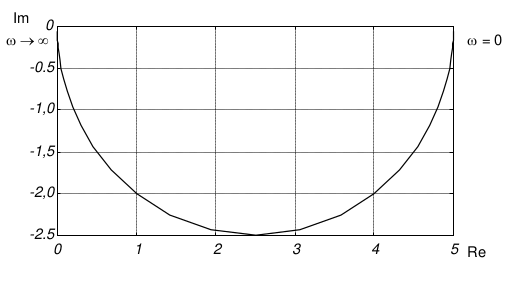
\includegraphics[width=.35\textwidth]{Figures/Ortskurve.png}
    \end{center}
    \begin{mdframed}[style=exercise]
    Für wachsendes $\omega$ werden die komplexen Werte F(j$\omega$) in die komplexe F-Ebene eingetragen und zur Ortskurve verbunden.\\
Jeder Ortskurvenpunkt kann jetzt als Zeiger gedeutet werden.\\
\end{mdframed}
    Bodediagrammdarstellung:
    \begin{center}
        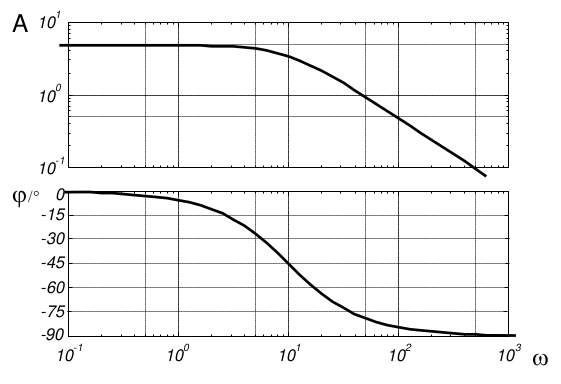
\includegraphics[width=.35\textwidth]{Figures/Bodediagramm.png}
    \end{center}
    \begin{mdframed}[style=exercise]
    Der Amplitudengang A($\omega$) wird in doppeltlogarithmischer Darstellung aufgetragen,\\
    der Phasengang y($\omega$)) halblogarithmisch. Gemeinsame Abszisse ist $\omega$.\\
    Bei diesem Beispiel (PT1-Glied) ist deutlich der Tiefpass-Charakter zu erkennen.\\
    Verkettete Funktionen im Bodediagramm resultieren als Produkt der Einzelübertragungsfunktionen.\\
    D.h. Verstärkung wird multipliziert und Phasenverschiebung addiert.
    Das heißt: Sowohl Phasengang (halblogarithmische Darstellung) und Amplitudengan (logarithmische Darstellung) werden graphisch addiert!
\end{mdframed}
\subsection{F(s) in Pol- und Nullstellenform}
\begin{mdframed}[style=exercise]
        Zähler- und Nennerpolynom von F(s) besitzt Nullstellen. Diese sind von $a_v$ und $b_u$ abhängig.\\
        Nullstellen des Zählers sind Nullstellen von F(s)\\
        Nullstellen des Nenners sind Polstellen von F(s)\\
        Wenn Pole $s_pv$ und Nullstellen $s_nu$ bekannt, kann man F(s) mit dem Faktor Q in faktorisierter Form darstellen.
    \end{mdframed}
    \begin{center}
            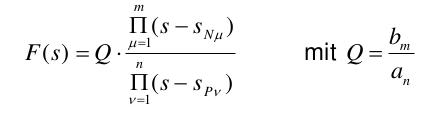
\includegraphics[width=.35\textwidth]{Figures/PolNullstellenQ.png}
        \end{center}
        \begin{mdframed}[style=exercise]
        Die Stabilität von F(s) kann anhand der Lage der Pole $s_pv$ in der s-Ebene beurteilt werden.\\
        F(s) ist stabil, wenn alle Pole $s_pv$ in der linken s-Halbebene liegen.\\
        Instabile Pole in der Rechten Halbebene lassen sich nicht durch Reihenschaltung
         mit entsprechender Nullstelle kompensieren!
    \end{mdframed}
    \begin{mdframed}[style=exercise]
        Bedeutung Polstelle:\\
        Pole bewirken ein zeitverzögertes Verhalten. je weiter links sie sich befinden,
        desto schneller ist der Einschwingvorgang.\\
        => Wenn Pole deutlich weiter links liegen als andere andere, kann man sie ohne
        großen Fehler vernachlässigen.\\
    \end{mdframed}
    \begin{mdframed}[style=exercise]
        Bedeutung Nullstelle:\\
        NS bewirken ein differenzierendes Verhalten (Beschleunigung des Systems)
        Einfluss weit links in der s-Ebene kann häufig vernachlässigt werden.

    \end{mdframed}
\subsection{Signalflussplanalgebra}
    Kettenstruktur:\\
    \begin{center}
            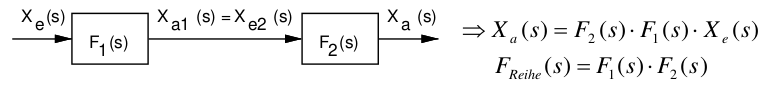
\includegraphics[width=.45\textwidth]{Figures/Kettenstruktur.png}
    \end{center}
    Parallelstruktur:\\
    \begin{center}
                    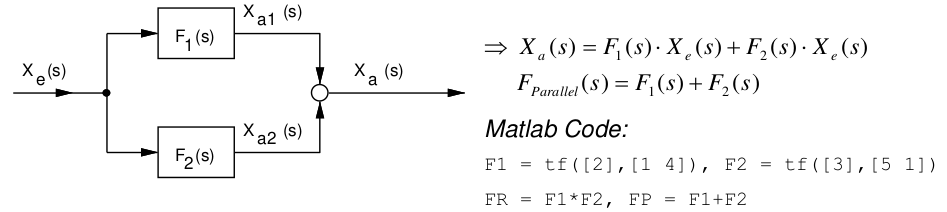
\includegraphics[width=.45\textwidth]{Figures/Parallelstruktur.png}
    \end{center}
    Kreisstruktur:\\
    \begin{center}
                    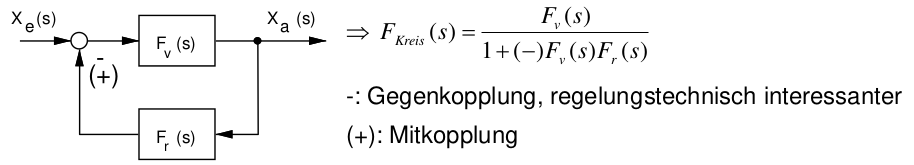
\includegraphics[width=.5\textwidth]{Figures/Kreisstruktur.png}
    \end{center}
    Verschieben einer Additionsstelle:\\
    \begin{center}
                    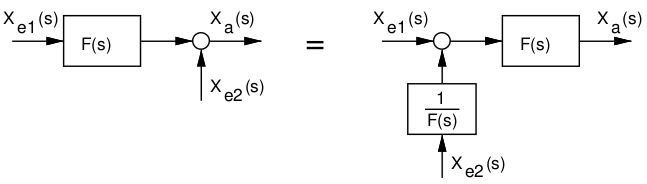
\includegraphics[width=.45\textwidth]{Figures/Verschiebung einer Additionsstelel.png}
    \end{center}
    Verschieben einer Verzweigung:\\
    \begin{center}
                    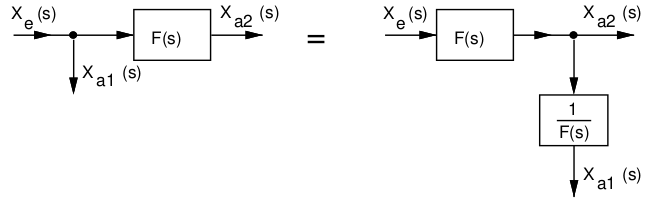
\includegraphics[width=.45\textwidth]{Figures/Verschiebung einer Verzweigung.png}
    \end{center}
\section{Zusammenwirken mehrerer Systeme}
  \subsection{Regelkreis}
  Anforderungen:
  \begin{mdframed}[style=exercise]
        Stabilität: Regelkreis muss stabiles Verhalten zeigen (gilt auch für instabile Systeme)\\
        Gutes Führungsverhalten: Die Differenz zw. Sollwert w(t) und Istwert x(t) muss schnell klein werden.\\
        Gutes Störverhalten: Einfluss von Störgrößen soll vermindert werden.
  \end{mdframed}
  Grundstruktur deseinschleifigen Regelkreises

  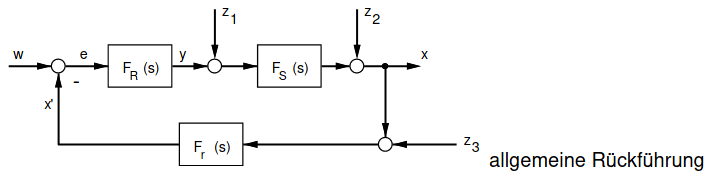
\includegraphics[width=.45\textwidth]{Figures/einschleifiger Regelkreis.png}

  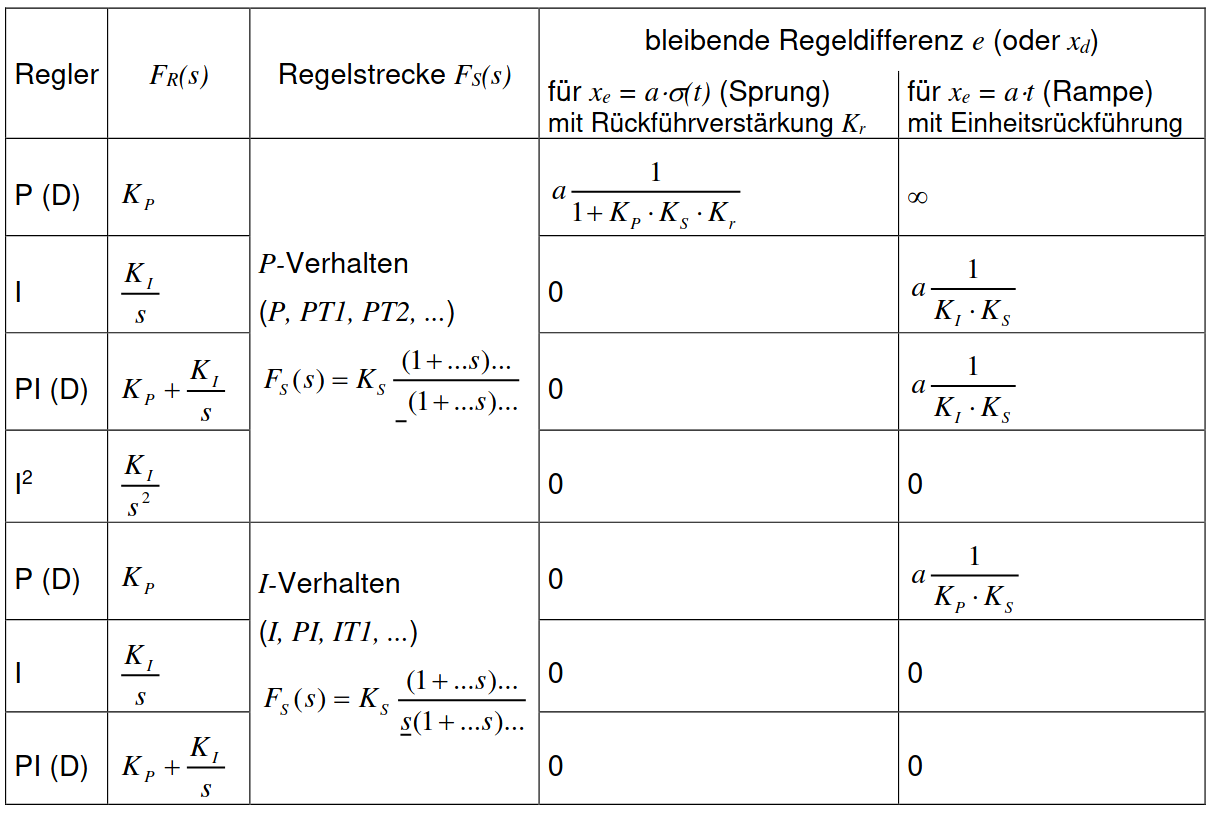
\includegraphics[width=.45\textwidth]{Figures/Reglerauswahl.png}


  \subsection{Wurzelortskurven (WOK)-Verfahren}
  \begin{mdframed}[style=exercise]
      Reglerfunktion $F_R$ in Reglerverstärkung und Reglerdynamik aufspalten:
      $F_R =K \cdot F_R ' $\\
  \end{mdframed}
  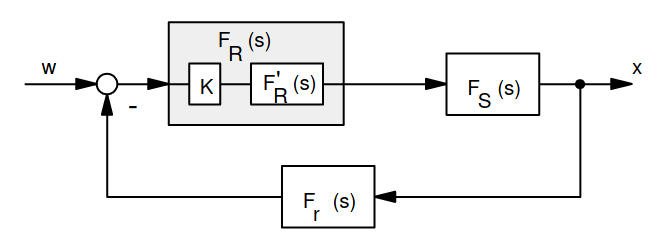
\includegraphics[width=.45\textwidth]{Figures/WOKkreis.png}
  \[
  \Rightarrow F_w (s)= \dfrac {F_R \cdot F_S} {1+F_R \cdot F_S \cdot F_r}\]
       \begin{mdframed}[style=exercise]

     Dabei ist $F_o = F_R \cdot F_S \cdot F_r$ die Übertragungsfunktion des offenen Regelkreises.
    $F_o$ kann auch in faktorisierter Form angegeben werden:
  \end{mdframed}
  \begin{align*}
  F_w (s)&= F_R (s) \cdot F_S (s) \cdot F_r (s)\\
        &=K \cdot F_R '(s) \cdot F_S (s) \cdot F_r (s)\\
        &=K \cdot Q \cdot \frac{\prod_{u=1}^{m}\left(s-s_{\text {Nou }}\right)}{\prod_{v=1}^{n}\left(s-s_{\text {pov }}\right)}
  \end{align*}
  Für eine Polstele, muss der Nenner von $F_w (s)$ Null werden:
  \[ \dfrac{F_R (s) \cdot F_S (s)}{1+F_o (s)} \Rightarrow 1+F_o (s) \stackrel{!}{=}0\]
  Daraus folgt:
  \begin{align*}
      &\Rightarrow 1+ K \cdot Q \cdot \frac{\prod_{M=1}^{m}\left(s-s_{\text {Nou }}\right)}{\prod_{v=1}^{n}\left(s-s_{\text {por }}\right)}\\
      &\Rightarrow \frac{\prod_{v=1}^{n}\left(s-s_{\text {pov }}\right)}{\prod_{u=1}^{m}\left(s-s_{\text {Nou }}\right)} \stackrel{!}{=} -K \cdot Q
  \end{align*}

  \subsection{Konstruktion der WOK}
  \begin{mdframed}[style=exercise]
      \begin{enumerate}
        \item Alle n Äste der WOK beginnen mit K=0 in den n Polen $s_pov$ des offenen Regelkreises.\\
        \item m Äste der WOK enden für K $\rightarrow \pm \infty$
        \item n -m Äste der WOK enden für K $\rightarrow \pm \infty$ im Unendlichen
        \item Die n-m ins Unendliche strebende Äste der WOK haben Asymptoten,die\\
            a) im Wurzelschwerpunkt
            \[S_{w}=\frac{\sum_{v=1}^{n} s_{pov}-\sum_{u=1}^{m} s_{_{Nop}}}{n-m}\]
            beginnen und die dabei\\
            b) mit der reellen Achse die Winkel\\
            $\varphi_{k}=\frac{(2 k-1) \cdot 180^{\circ}}{n-m}$ für KQ > 0 bzw.
            $\varphi_{k}=\frac{(2 k-2) \cdot 180^{\circ}}{n-m}$ für KQ < 0 \\
            mit k = 1,2,3,\dots,n-m
        \item Die Punkte der WOk liegen entweder auf der reelen Achse, oder symmetrisch zur reelen Achse
        \item Ein Punkt s auf der reellen Achse ist dann ein Punkt der WOK, wenn sich bei KQ > 0 (KQ<0)
            rechts von ihm eine ungerade (gerade) Anzahl von Polen $s_{pov}$ und (+) Nullstellen $s_{Nov}$ befindet.
\end{enumerate}
Achtung: WOK ist nicht anwendbar, wenn es sich um nicht rationale Übertragungsfunktionen handelt.
 (z.B. Regelkreis mit Totzeitverhalten!)
  \end{mdframed}
\subsection{Nyquist Kriterium}
    \begin{center}
      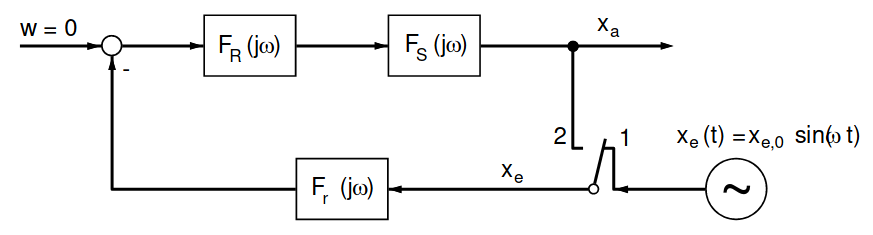
\includegraphics[width=.45\textwidth]{Figures/Nyquist.png}
    \end{center}
    Frequenzgangfunktion des offenen Regelkreises:
    \[ F_o (j\omega) = F_r (j\omega) \cdot F_R (j\omega) \cdot F_S (j\omega)\]
    Ausgangssignal:
    \[ x_a(t)=-F_r (j\omega) \cdot F_R (j\omega) \cdot F_S (j\omega) \cdot x_{e0} sin(\omega t)=
    -F_0 (j\omega) \cdot x_e (t)\]
    Regler und seine Parameter werden so gewählt, dass $\omega = \omega_{krit}$ gilt:
    \[-F_0 (j\omega_{krit})=1 \text{ oder } F_0 (j\omega_{krit})=-1 \text{ (Schwingbedingung)}\]\
    \begin{mdframed}[style=exercise]
        Die Schwingbedingung ist erfüllt, wenn die Ortskurve von $F_1 (j\omega)$ durch den kritischen
        Punkt ($P_{krit} = -2+j0$) der komplexen $F_0$-Ebene geht. An diesem Punkt kann man
        $\omega_{krit}$ ablesen (damit kann der Regelkreis Dauerschwingungen ausführen).
        Für gößere $\omega$ ist das System instabil, für kleinere stabil.



    \end{mdframed}
    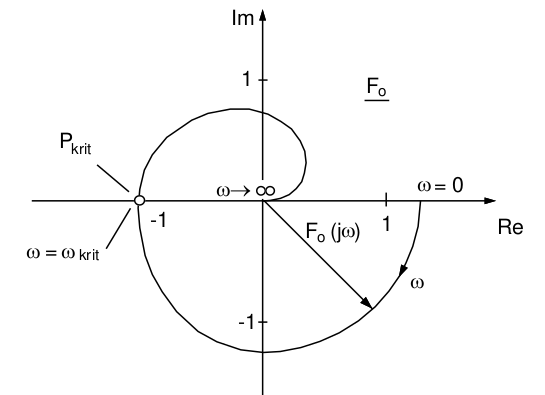
\includegraphics[width=.45\textwidth]{Figures/Nyquistwkrit.png}
    \begin{mdframed}[style=exercise]
        Falls F(s) des offenen Kreises keine Pole in der rechten Halbebene hat und nur max. 2 im Ursprung der s-Ebene,
        ist der Regelkreis stabil, wenn der kritische Punkt von $\omega$ immer links von
        s = -1 + 0j liegt. (gilt immer wenn der offene Kreis stabil ist)
    \end{mdframed}
    Zur Auswertung des Nyquist-Kriteriums im Bode Diagramm, spaltet man die Ortskurve nach Betrag
    A = |$F_0 (jw)$ und Phase $\varphi$ = $F_0(jw)$\\
    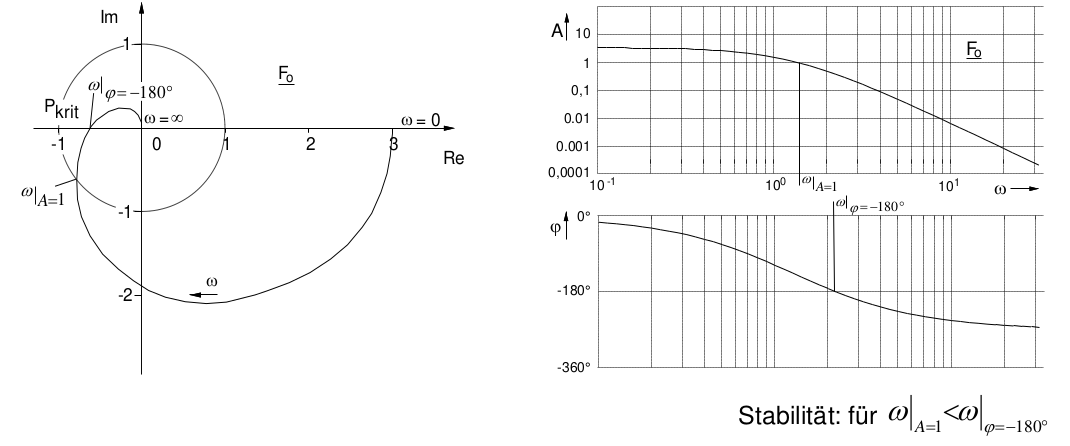
\includegraphics[width=.5\textwidth]{Figures/Nyquist_Bode.png}
    Falls die Bedingung nicht funktioniert, wird die allgemene Formulierung verwendet:\\
    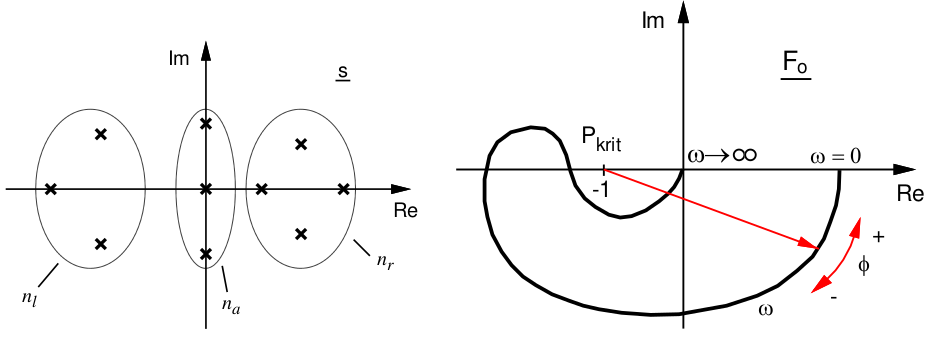
\includegraphics[width=.5\textwidth]{Figures/Allgemein_Nyquist.png}

\section{Grundlagen}
  \subsection{Eigenschaften}
  Eigenschaften LTI-Systeme die Ortskurve von $F_-1 (j\omega)$ durch den kritischen
  Punkt ($P_{krit} = -2+j0$)der komplexen $F_0$-Ebene
  \begin{mdframed}[style=exercise]
    \begin{enumerate}
      \item Stabilität\\
      $\abs{x(t)} < M < \infty \Rightarrow \abs{y(t)} < N < \infty$
      \item Linearität\\
      $W\qty{\sum_{k=1}^{N}a_n x_n(t)}=\sum_{n=1}^{N}W\qty{a_n x_n(t)}$
      \item Zeitinvarianz\\
      $W\qty{x(t-t_0)} =y(t-t_0)$
      \item Kausalität\\
      $t < 0 \Rightarrow x(t)=0 \land y(t)=0$
    \end{enumerate}
  \end{mdframed}
  \subsection{Systemantwort}
  Die Sprung-/Impulsantwort beschreibt Systemantwort vollständig
  \begin{mdframed}[style=exercise]
    \begin{align}
      y(t) &= \int^{\infty}_{-\infty} a(t-\tau) x'(\tau) \dd{\tau}\\
      a(t-\tau) &= W\qty{s(t-\tau)}\nonumber
    \end{align}
  \end{mdframed}
  \begin{mdframed}[style=exercise]
    \begin{align}
      y(t) &= \int_{-\infty}^{\infty} h(t-\tau) x(\tau) \dd{\tau}\\
      h(t-\tau) &= W\qty{\delta(t-\tau)}\nonumber
    \end{align}
  \end{mdframed}
  \subsection{Abtasttheorem}
  Durch die Abtastung wird das Spektrum von $f(t)$ unendlich oft um die Frequenzen $n\cdot \omega_a$ reproduziert.
  \begin{mdframed}[style=exercise]
    \begin{align}
      F_A(\omega) &= \frac{1}{T_A} \sum_{n=-\infty}^{\infty} F(\omega-n\omega_A)\\
      2\omega_g &\leq \omega_A\nonumber
    \end{align}
  \end{mdframed}
  \section{Zusammenwirken mehrerer Systeme}
  \subsection{Fourierreihe}
  \begin{mdframed}[style=exercise]
    \begin{align}
      f(t) &= \sum_{n=0}^{\infty} \qty[a_n \cos(n \omega_0 t) + b_n \sin(n \omega_0 t)]\\
      a_n &= \frac{2}{T}\int_{-T/2}^{T/2}f(t)\cos(n\omega_0 t)\dd{t}\nonumber\\
      b_n &= \frac{2}{T}\int_{-T/2}^{T/2}f(t)\sin(n\omega_0 t)\dd{t}\nonumber
    \end{align}
  \end{mdframed}
  \pagebreak
  \subsection{Fourierreihe, komplex}
  \begin{mdframed}[style=exercise]
    \begin{align}
      f(t) &= \sum_{n=-\infty}^{\infty} c_n e^{jn\omega_0 t}\\
      c_n &= \frac{1}{T} \int_{-T/2}^{T/2} f(t) e^{-jn\omega_0 t}\dd{t}\nonumber
    \end{align}
  \end{mdframed}
  \subsection{Fourierintegral}
  \begin{mdframed}[style=exercise]
    \begin{align}
      f(t) &= \frac{1}{2\pi} \int_{-\infty}^{\infty} F(\omega) e^{j\omega t} \dd{\omega}\\
      F(\omega) &= \int_{-\infty}^{\infty} f(t) e^{-j\omega t} \dd{t}
    \end{align}
  \end{mdframed}
  \subsubsection{Eigenschaften}
  \begin{mdframed}[style=exercise]
    \begin{enumerate}
      \item Linearität\\
      $a f_1(t) + b f_2(t) \laplace a F_1(\omega) + b F_2(\omega)$
      \item Zeitverschiebung\\
      $f(t-t_0) \laplace F(\omega)e^{-j\omega t_0}$
      \item Frequenzverschiebung\\
      $f(t) e^{\pm j\omega_0 t}\laplace F(\omega\mp \omega_0)$
      \item Faltung\\
      $f_1(t)*f_2(t)\laplace F_1(\omega)\cdot F_2(\omega)$\\
      $f_1(\omega)\cdot f_2(\omega)\laplace \frac{1}{2\pi}F_1(t)*F_2(t)$
    \end{enumerate}
  \end{mdframed}
  \subsection{DFT}
  \begin{mdframed}[style=exercise]
    \begin{align}
      x_n &= \frac{1}{N} \sum_{k=0}^{N-1} X_k\cdot e^{i 2 \pi k n / N}\\
      X_k &= \sum_{n=0}^{N-1} x_n\cdot e^{-i 2 \pi k n / N}
    \end{align}
  \end{mdframed}
  \subsubsection{FFT}
  \begin{center}
    \includegraphics[width=.35\textwidth]{Figures/butterfly}
    \captionof{figure}{FFT}
  \end{center}
  \pagebreak
  \subsection{Hilbert Transformation}
  \begin{mdframed}[style=exercise]
    \begin{align}
      x_{\mathrm{ht}}(t) &= x_{\mathrm{r}}(t) * h(t)\\
      H(\omega) &= -j \, \text{sgn}(\omega)
    \end{align}
  \end{mdframed}
  \subsection{z Transformation}
  \begin{mdframed}[style=exercise]
    \begin{align}
      X(z) &= \sum_{n=-\infty}^{\infty} x(n) z^{-n}\\
      x(n) &= \frac{1}{2\pi j} \oint_c X(Z) z^{n-1}\dd{z}
    \end{align}
  \end{mdframed}
  \subsubsection{Übertragungsfunktion}
  \begin{mdframed}[style=exercise]
    \begin{align}
      H(Z) &=\frac{Y(Z)}{X(z)}=\frac{\sum_{k=0}^q b_k z^{-k}}{\sum_{k=0}^p a_k z^{-k}}=k\frac{\prod_{k=1}^q (1-z_k z^{-1})}{\prod_{k=1}^p (1-p_k z^{-1})}
    \end{align}
  \end{mdframed}
  \subsubsection{Verschiebung im Zeitbereich}
  \begin{mdframed}[style=exercise]
    \begin{align}
      Y(z) &= \sum_{n=0}^{\infty} \qty[x(n-m)] z^{-n} =  z^{-m} X(z)\\
      Y(z) &= \sum_{n=0}^{\infty}\qty[x(n+m)]z^{-n} = z^{m}\qty[x(t)-\sum_{n=0}^{m-1} x(n) z^{-n}]
    \end{align}
  \end{mdframed}
  \section{Digitale Regler}
  \subsection{FIR}
  \begin{mdframed}[style=exercise]
    \begin{align}
      y[n] &= \sum_{k=0}^{q} b_k x(n-k)
    \end{align}
  \end{mdframed}
  \begin{center}
    \includegraphics[width=.4\textwidth]{Figures/fir.png}
  \end{center}
  \subsection{IIR}
  \begin{mdframed}[style=exercise]
    \begin{align}
      y[n] &= \sum_{k=0}^{q} b_k x(n-k) - \sum_{k=1}^{p} a_k y(n-k)
    \end{align}
  \end{mdframed}
  \begin{center}
    \includegraphics[width=.35\textwidth]{Figures/df1.png}
    \captionof{figure}{Direkt Form 1}
  \end{center}
  \begin{center}
    \includegraphics[width=.35\textwidth]{Figures/df2.png}
    \captionof{figure}{Direkt Form 2}
  \end{center}
  \section{Systembeschreibung im Zustandsraum}
  \subsection{Allgemein (Mehrgrößensystem MIMO) }
  \begin{mdframed}[style=exercise]
    \begin{equation}
      \dot{\Vec{x}}(t) = A\vec{x}(t) + B\vec{u}(t); \quad x(0) = x_{0}; \\*
      \vec{y}(t) = C\vec{x}(t) + D\vec{u}(t)
    \end{equation}
  \end{mdframed}
  \begin{center}
    \includegraphics[width=.5\textwidth]{Figures/Signalflussplan.png}
    \captionof{figure}{Signalflussplan}
  \end{center}
  \begin{mdframed}[style=exercise]
    \begin{align*}
      \dot{x}_{1} &= 0*x_{1} +0*x_{2} +0*x_{3} +1*u_{1}+0*u_{2} \\
      \dot{x}_{2} &= K*x_{1} +0*x_{2} +0*x_{3} +0*u_{1}+0*u_{2} \\
      \dot{x}_{3} &= 0*x_{1} +0*x_{2} +0*x_{3} +H*J*u_{1}+J*u_{2} \\
      \dot{y}_{1} &= 0*x_{1} +1+x_{2} +0*x_{3} +0*u_{1}+0*u_{2} \\
      \dot{y}_{2} &= 0*x_{1} +0*x_{2} +l*x_{3} +0*u_{1}+0*u_{2} \\
    \end{align*}
  \end{mdframed}

  \begin{mdframed}[style=exercise]
   \[
        \ A = \begin{bmatrix}
            0&0&0\\
            K&0&0\\
            0&0&0
        \end{bmatrix}
        C = \begin{bmatrix}
            0&1&0\\
            0&0&l\\
        \end{bmatrix}\]\\
        \[B = \begin{bmatrix}
            1&0\\
            0&0\\
            H\cdot{}J&J
        \end{bmatrix} \
        D = \begin{bmatrix}
            0&0\\
            0&0
        \end{bmatrix}\]

  \end{mdframed}
  \subsection{Programmtechnische Umsetzung}
Zaehler und Nenner der z-Uebertragungsfunktion durch die hoechste Potenz teilen\\
  \begin{mdframed}[style=exercise]
    \begin{lstlisting}
      while(1){
      waitinterrupt();
      xout2 = xout1;
      xout1 = xout;
      xin2 = xin1;
      xin1 = xin;
      input(xin);
      xout = k*xout2 - j*xin1 + o*xout1;
      output(xa);
      }
    \end{lstlisting}
  \end{mdframed}
\end{document}
